\section{Identifikation der Reaktionsprodukte mithilfe von LC-MS}

Die Produkte der Reaktion mit Essigsäureanhydrid konnten ebenfalls mithilfe von \gls{lcms} identifiziert werden. In Abbildung \ref{fig:HPLCChromatogrammRP} sind die Reaktionsprodukte, die mittels UV/Vis online Spektren identifiziert wurden, dargestellt. Die dazugehörigen UV/Vis Spektren werden in Abbildung \ref{fig:YCC3398}-e dargestellt. Es handelt sich dabei um die Hauptreaktionsprodukte, die dadurch charakterisiert sind, dass sich ihre Retentionszeit nach hinten verschiebt. Sie dürften somit apolarere Eigenschaften besitzen wie die \gls{Chl-K}, was vermutlich durch den Methylester bedingt ist. Über die Verschiebung der Peaks im \gls{hplc} Chromatogramm ist das Stattfinden der Reaktion ersichtlich (vergleiche Abbildung \ref{fig:HPLCChromatogramm} und Abbildung \ref{fig:HPLCChromatogrammRP}). Es konnten mehrere Verbindungen über UV/Vis Spektren beobachtet und identifiziert werden wie bei den anderen \gls{hplc} Läufen.

\begin{figure}[!htbp]
  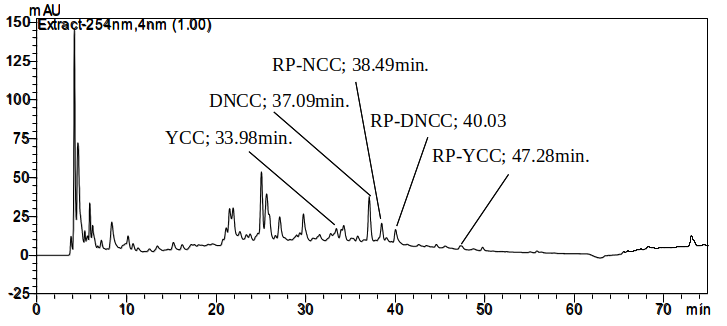
\includegraphics[width=\textwidth]{figures/Kapitel6/Reaktion3h/HPLC_Chromatogramm.png}
  \caption[HPLC Chromatogramm nach 3h Reaktionsdauer, Quelle: Author]{\gls{hplc} Chromatogramm}
  \label{fig:HPLCChromatogrammRP}
\end{figure}

Das Chromatogramm des Massenspektrometers des \gls{lcms} Laufes (Abbildung \ref{fig:LCMSCChromatogrammRP}) zeigt die Massen aller \gls{Chl-K} und die Zeitpunkte, zu denen sie jeweils eluieren. Durch die stattgefundene Reaktion sind dementsprechend mehr Signale vorhanden. Auffallend ist, dass manche Verbindungen in ihren Retentionszeiten verschoben worden sind. So eluiert Verbindung mit m/z = 631 [M+H]\textsuperscript{+} nun bei 39.0min. im Vergleich zu 18.9min., Verbindung mit m/z = 629 [M+H]\textsuperscript{+} bei 31.8min. im Vergleich zu 21.6min. und Verbindung mit m/z = 645 [M+H]\textsuperscript{+} bei 34.5min. im Vergleich zu 29.0min. (vergleiche Abbildung \ref{fig:LCMSCChromatogrammRP} und \ref{fig:LCMSChromatogramm}). Gründe für diese Verschiebung müssten weiter untersucht werden bzw. müsste überprüft werden, ob es bei den Versuchen, aus denen einer zu Abbildung \ref{fig:LCMSChromatogramm} führte, nicht einen Messfehler gab. Eine Überprüfung und erneute Durchführung der Messung führte jedoch zum selben Ergebnis (siehe Anhang).

\begin{figure}[!htbp]
  \centering
  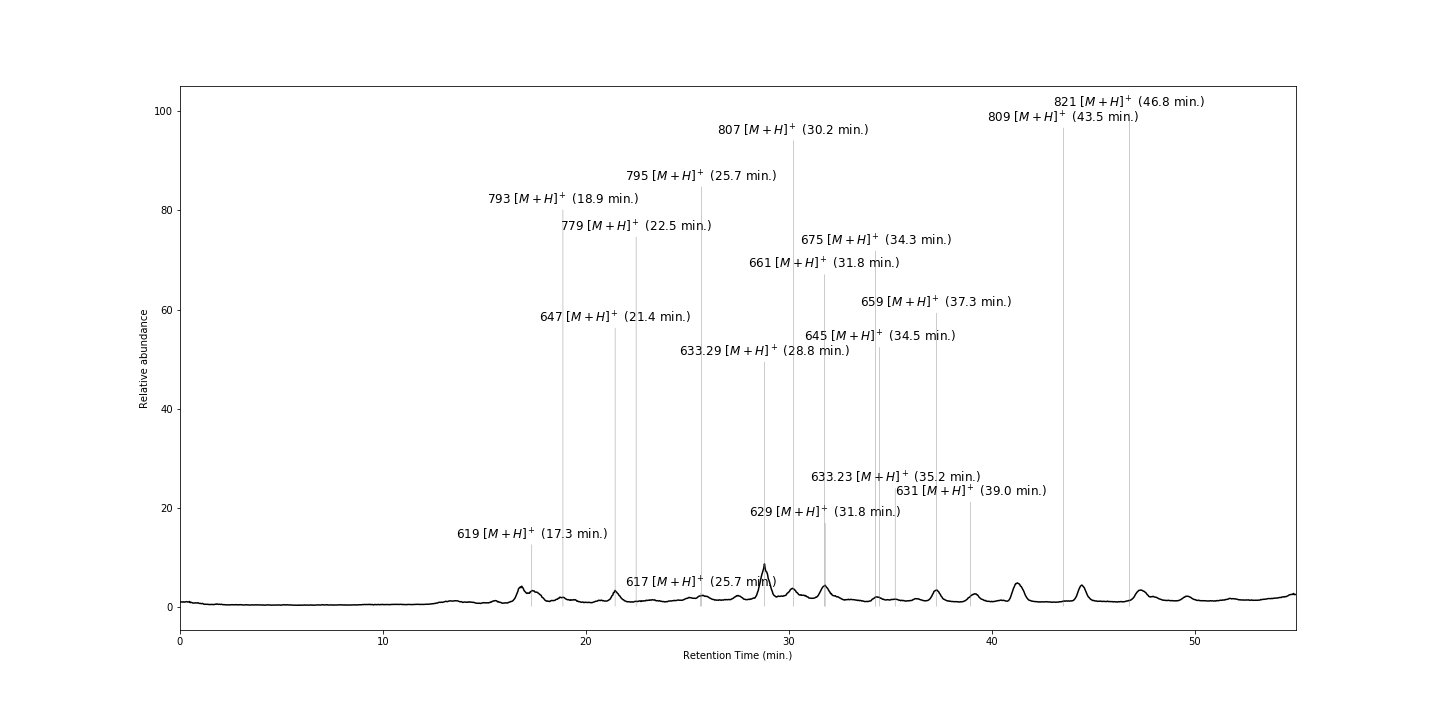
\includegraphics[width=1.1\textwidth]{figures/Kapitel6/Reaktion3h/Kuerbis_Analyse_Reaktion3h_Ganzes_Spektrum.png}
  \caption[LC-MS Chromatogramm nach 3h Reaktionsdauer, Quelle: Author]{\gls{lcms} Chromatogramm}
  \label{fig:LCMSCChromatogrammRP}
\end{figure}

In Tabelle \ref{tab:LCMSKatabolitenRP} werden die \gls{Chl-K} dargestellt, die nach der Reaktion gefunden wurden. Dabei wurden zwei Verbindungen entdeckt, die ähnliche Molekülmassen aufweisen, wie bereits identifizierte, 
\begin{table*}\centering
  \ra{1.3}

  \begin{tabular}{cccccc}\toprule
 Bezeichnung & Summenformel & M (in Da) & Typ & RT\textsubscript{HPLC} (in min.) & H. \\
\midrule
\rowcolor{black!20} Bo-DYCC & \ch{C33H37O8N4} & 617.2599 & DYCC & 30.94? & - \\
 Bo-DNCC & \ch{C33H39O8N4} & 619.2798 & DNCC & 26.72 & - \\ 
\rowcolor{black!20} • & \ch{C34H37O8N4} & 629.2641 & • & - & - \\ 
 - & \ch{C34H39O8N4} & 631.2795 & DYCC & 29.91, 30.94 & Bo-DYCC \\ 
\rowcolor{black!20} - & \ch{C34H41O8N4} & 633.2955 & DNCC & 28.8 & Bo-DNCC \\ 
 • & \ch{C36H33O7N4} & 633.2339 & • & - & - \\ 
\rowcolor{black!20} Bo-YCC & \ch{C34H37O9N4} & 645.2593 & YCC & - & - \\ 
 • & \ch{C35H41O8N4} & 645.2953 & • & - & - \\ 
\rowcolor{black!20} Bo-NCC-3 & \ch{C34H39O9N4} & 647.2748 & NCC & 33.04 & - \\ 
 • & \ch{C34H35O10N4} & 659.2348 & • & - & - \\
\rowcolor{black!20} - & \ch{C35H39O9N4} & 659.2741 & YCC & 37.09 & Bo-YCC \\
 - & \ch{C35H41O9N4} & 661.2902 & - & - & Bo-NCC-3 \\
\rowcolor{black!20} - & \ch{C36H43O9N4} & 675.306 & - & - & Bo-NCC-3 \\
 Bo-DNCC-2 & \ch{C39H47O13N4} & 779.3181 & DNCC & - & - \\ 
\rowcolor{black!20} Bo-NCC-1 & \ch{C40H49O13N4} & 793.3336 & NCC & 29.91 & - \\ 
 - & \ch{C40H51O13N4} & 795.3491 & - & - & - \\ 
\rowcolor{black!20} - & \ch{C41H51O13N4} & 807.3491 & NCC & 40.03 & Bo-NCC-1 \\ 
 - & \ch{C41H53O13N4} & 809.3649 & - & - & 795 \\ 
\rowcolor{black!20} - & \ch{C42H53O13N4} & 821.3652 & NCC & 47.28 & Bo-NCC-1 \\ 
\bottomrule
  \end{tabular}
  \caption[Übersicht über die Chl-Kataboliten des Brokkoliblattes, Quelle: Author]{Übersicht über die gefundenen Chl-Kataboliten des Brokkoliblattes und ihren Methylestern, die sich aus der Reaktion der freien Carbonsäure mit Essigsäureanhydrid und der anschließenden Aufarbeitung mit \gls{meoh} ergeben. Durch die Aktivierung der Reaktion sind mehr Produkte zu sehen und diese sind in größeren Intensitäten vorhanden. (die Summenformeln und die exakten Molekülmassen beziehen sich auf die [M+H]\textsuperscript{+} Ionen)}
  \label{tab:LCMSKatabolitenRP}
\end{table*}


\begin{figure}[!htbp]
  \begin{subfigure}[b]{0.5\textwidth}
    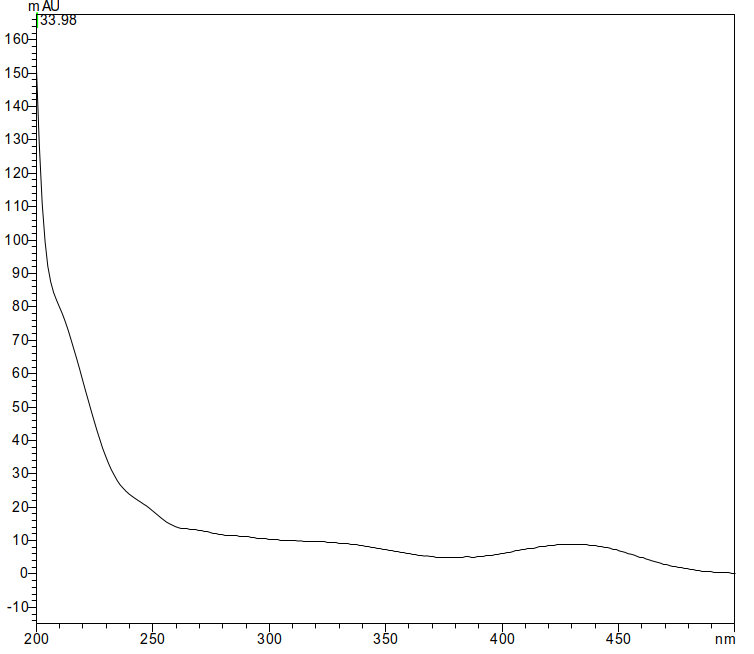
\includegraphics[width=\textwidth]{figures/Kapitel6/Reaktion3h/YCC3398.png}
    \caption{}
    \label{fig:YCC3398}
  \end{subfigure}
  \hfill
  \begin{subfigure}[b]{0.5\textwidth}
    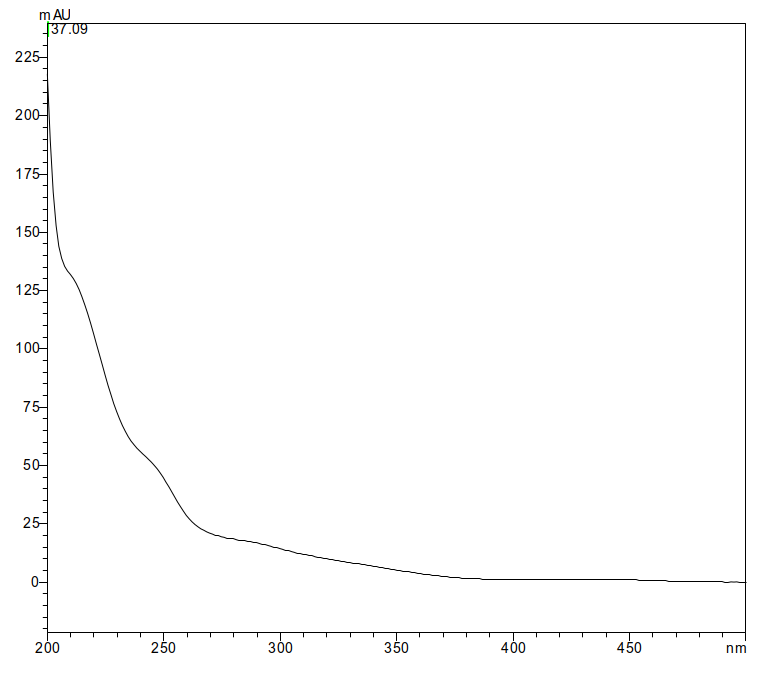
\includegraphics[width=\textwidth]{figures/Kapitel6/Reaktion3h/DNCC3709.png}
    \caption{}
    \label{fig:DNCC3709}
  \end{subfigure}
  
  \begin{subfigure}[b]{0.5\textwidth}
    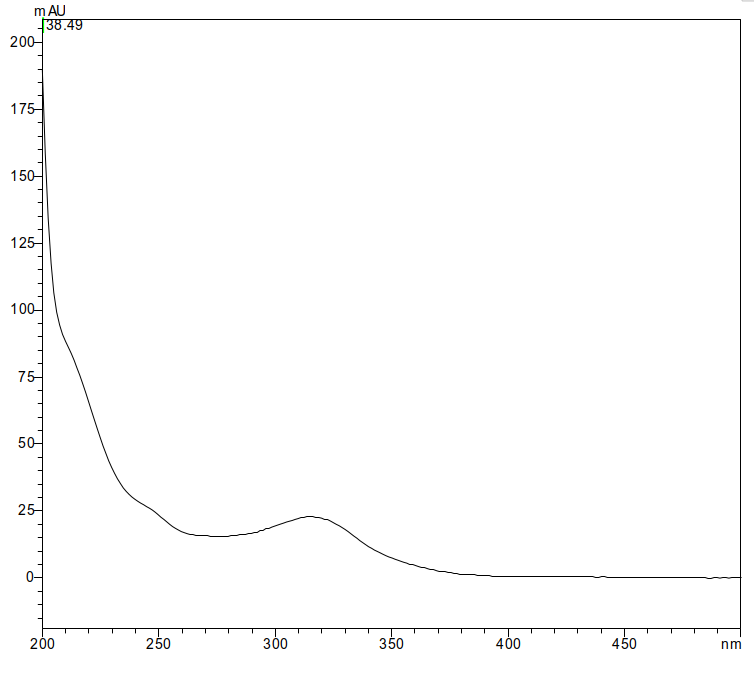
\includegraphics[width=\textwidth]{figures/Kapitel6/Reaktion3h/NCC3849.png}
    \caption{}
    \label{fig:NCC3849}
  \end{subfigure}
  \hfill
  \begin{subfigure}[b]{0.5\textwidth}
    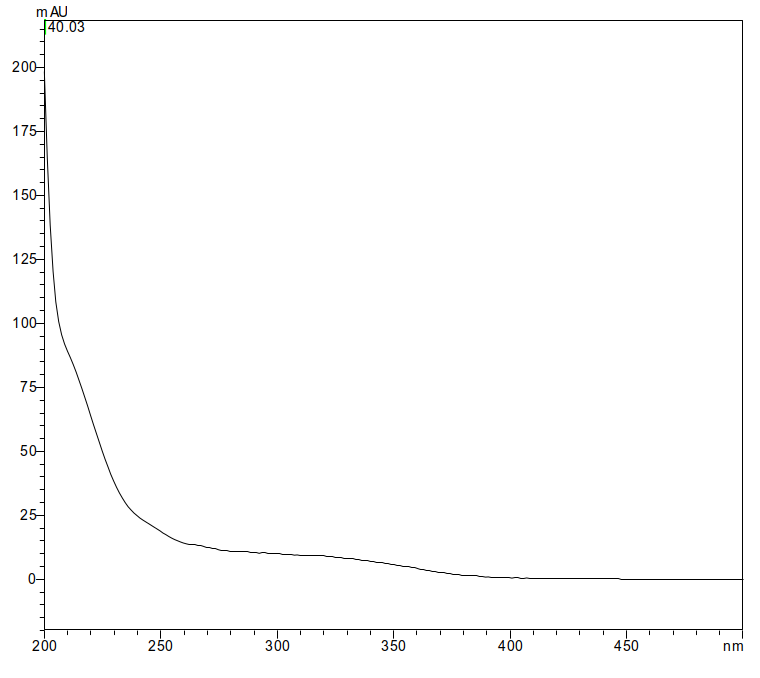
\includegraphics[width=\textwidth]{figures/Kapitel6/Reaktion3h/DNCC4003.png}
    \caption{}
    \label{fig:DNCC4003}
  \end{subfigure}
  
  \begin{subfigure}[b]{0.5\textwidth}
    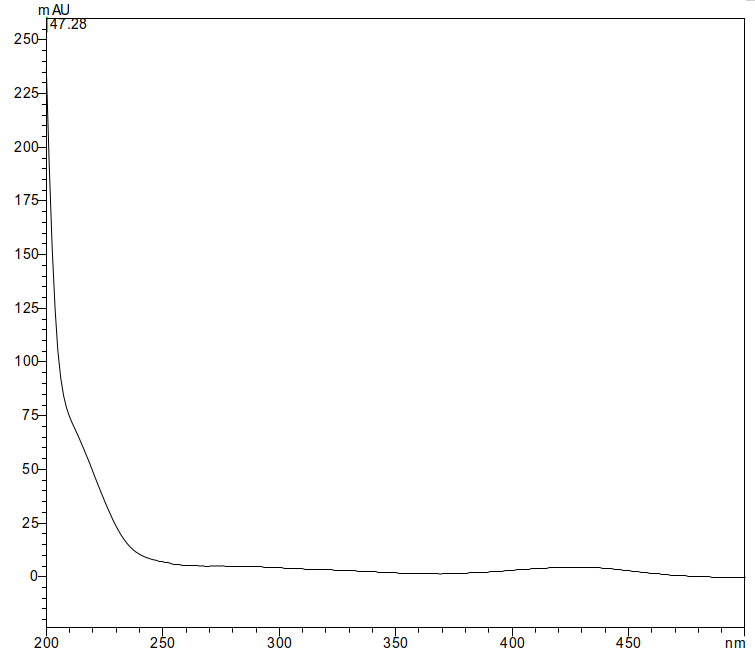
\includegraphics[width=\textwidth]{figures/Kapitel6/Reaktion3h/YCC4728.png}
    \caption{}
    \label{fig:YCC4728}
  \end{subfigure}
  \caption[UV/Vis online Spektren mit der Charakteristik eines YCC bei 33.98min., eines DNCC bei 37.09min. eines NCC bei 38.94min., eines DNCC bei 40.03min. sowie eines YCC bei 47.28min., Quelle: Author]{UV/Vis online Spektren: charakeristisch für (a) \gls{YCC} - RT = 33.98min., (b) \gls{DNCC} - RT = 37.09min., (c) \gls{NCC} - RT = 38.94min., (d) \gls{DNCC} - RT = 40.03min., (e) \gls{YCC} - RT = 47.28min.}
\end{figure}

